\documentclass[conference]{IEEEtran}

% Idioma y codificación
\usepackage[utf8]{inputenc}
\usepackage[spanish]{babel}
\usepackage{csquotes}

% Matemáticas
\usepackage{amsmath, amsfonts, amssymb}

% Gráficos y tablas
\usepackage{graphicx}
\usepackage{booktabs}
\usepackage{multirow}
\usepackage{subcaption}
\usepackage{float}
\usepackage{tikz}
\usepackage{pgfplots}
\usetikzlibrary{positioning, arrows.meta}

% Algoritmos
\usepackage{algorithm}
\usepackage{algorithmic}

% Enlaces
\usepackage{hyperref}
\hypersetup{
    colorlinks=true,
    linkcolor=black,
    urlcolor=black,
    citecolor=black
}

% Citas
\usepackage[numbers,square,sort&compress]{natbib}

% Fuente
\usepackage{times}

% Comienzo del documento
\begin{document}

% TÍTULO Y AUTOR
\title{Algoritmos Evolutivos en Espacios de Alta Dimensionalidad para Optimización de Rutas}

\author{
    \IEEEauthorblockN{Yonhel Mamani Cruz}
    \IEEEauthorblockA{
        Facultad de Ingeniería Estadística e Informática\\
        Universidad Nacional del Altiplano\\
        Puno, Perú\\
        \href{72689624@est.unap.edu.pe}{72689624@est.unap.edu.pe}
    }
}

\maketitle

% RESUMEN
\begin{abstract}
La optimización de rutas a gran escala representa uno de los desafíos más complicados en el ámbito de la gestión de rutas, particularmente en la optimización combinatoria cuando se tratan espacios de búsqueda de alta dimensión.
En este estudio se realizó un análisis detallado sobre la efectividad de algoritmos evolutivos (AEs) aplicados a situaciones concretas del problema de ruteo con un máximo de 62 ciudades. Se examinaron metodologías como Algoritmos Genéticos (AG), Evolución Diferencial (ED) y Optimización por Enjambre de Partículas (OEP), en contraste con algoritmos evolutivos híbridos (AEH) diseñados para optimizar el balance entre la exploración y la explotación.
Los hallazgos experimentales mostraron que el AEH consiguió una mejora del 52.6\,\% en comparación con los métodos aleatorios convencionales, disminuyendo la distancia total de 73,593,576.9 a 34,892,902.0 unidades. Estos descubrimientos corroboran la literatura actual acerca de la superioridad de enfoques mixtos en espacios complejos \cite{talbi2002, sorensen2013}, y proporcionan implicaciones prácticas significativas en la logística y distribución a gran escala.
\end{abstract}

% PALABRAS CLAVE
\begin{IEEEkeywords}
algoritmos evolutivos, optimización combinatoria, ruteo, algoritmos híbridos, alta dimensionalidad.
\end{IEEEkeywords}

% INICIO DEL ARTÍCULO

\section{Introducción}

El Problema de Ruteo de Vehículos (PRV) y sus variantes han sido reconocidos como desafíos centrales dentro de la optimización combinatoria, con aplicaciones críticas en logística, transporte y la gestión de cadenas de suministro \cite{toth2014}. A medida que las redes logísticas modernas escalaron en complejidad y tamaño, la dimensionalidad de los problemas de ruteo aumentó exponencialmente, generando espacios de búsqueda altamente complejos conocidos como ``espacios de optimización de rutas de alta dimensionalidad''.

La motivación principal de este estudio surgió de la necesidad creciente de enfrentar la complejidad operativa de sistemas de distribución de gran escala. Empresas globales como Amazon, FedEx y UPS gestionan millones de entregas cada día, lo que demanda algoritmos de optimización capaces de explorar eficientemente espacios de solución con miles de variables. Los enfoques exactos, si bien teóricamente óptimos, se volvieron computacionalmente intratables para instancias que superan los 100 nodos \cite{applegate2007}. Esto condujo al desarrollo de métodos metaheurísticos, en particular aquellos de tipo evolutivo, por su capacidad para ofrecer soluciones de calidad en tiempos razonables \cite{blum2003}.

Desde una perspectiva práctica, la aplicación efectiva de estos algoritmos podría generar beneficios sustanciales, incluyendo reducciones de hasta 30\,\% en costos operacionales\cite{toth2014}, una menor huella ambiental debido a rutas más eficientes, y mejoras significativas en la puntualidad de las entregas y la satisfacción del cliente. Estas mejoras son especialmente relevantes en el contexto del crecimiento acelerado del sector logístico global durante las últimas décadas.

El presente estudio tuvo como propósito analizar el rendimiento de distintos algoritmos evolutivos aplicados a problemas de optimización de rutas de alta dimensionalidad. Se propuso el desarrollo de enfoques híbridos que integraran múltiples estrategias evolutivas, así como la evaluación de la escalabilidad de dichas técnicas frente a diversas configuraciones de problema. Finalmente, se buscó proporcionar evidencia empírica que respalde la selección de algoritmos eficientes en aplicaciones logísticas del mundo real.

\section{Revisión de Literatura}

Los algoritmos evolutivos han demostrado un éxito notable en la resolución de problemas de optimización complejos durante las últimas tres décadas \cite{fogel2006,back2013}. Encuestas recientes indican que la computación evolutiva es un campo en rápida evolución, y que los algoritmos relacionados se han utilizado exitosamente para resolver una amplia variedad de problemas del mundo real \cite{yang2013}. Este desarrollo responde a la necesidad de abordar problemas donde los métodos exactos tradicionales resultan insuficientes debido a su alta complejidad computacional.

El campo ha experimentado avances importantes en áreas como la optimización asistida por modelos sustitutos, diseñada para enfrentar el alto costo computacional de las evaluaciones de funciones \cite{jin2011}; la optimización multiobjetivo, que permite manejar simultáneamente objetivos conflictivos \cite{coello2007,zhang2008}; la optimización a gran escala, que enfrenta el reto de variables en el orden de los miles \cite{lozano2011}; y el diseño automatizado de algoritmos, que permite ajustes auto-adaptativos de parámetros durante la ejecución \cite{brest2006}. Estos desarrollos reflejan la evolución natural del campo hacia soluciones más robustas y escalables.

Dentro de contextos de alta dimensión, los algoritmos evolutivos se encuentran con retos considerables.
Debido al fenómeno denominado "la maldición de la dimensionalidad", donde el volumen del espacio de búsqueda aumenta de manera exponencial con el número de variables. Esto hace inviable la exploración exhaustiva y requiere enfoques inteligentes como los algoritmos evolutivos asistidos por sustitutos (AEAS), que han ganado atención por su capacidad de mitigar estos costos computacionales \cite{wang2018}.

En el contexto específico del Problema de Ruteo de Vehículos (PRV), estudios anteriores han reportado resultados prometedores usando algoritmos evolutivos. Sin embargo, la mayoría de estas investigaciones se limitaron a instancias de pequeña a mediana escala \cite{rego2011}. La literatura actual muestra una brecha crítica en la comprensión del comportamiento de estos algoritmos en contextos de gran escala, especialmente cuando el número de nodos supera los miles. Esta limitación ha motivado el desarrollo de enfoques híbridos, que combinan las fortalezas de múltiples paradigmas evolutivos para lograr un balance eficiente entre exploración y explotación del espacio de búsqueda \cite{potter2000}.


\section{Marco Teórico}

La optimización de rutas representa una de las problemáticas más estudiadas en la investigación operativa y computación evolutiva, modelada clásicamente como el Problema del Viajante (TSP) o el Problema de Ruteo de Vehículos (VRP). Estos problemas son NP-duros, por lo cual el uso de algoritmos exactos se vuelve inviable para instancias grandes. En consecuencia, se han adoptado estrategias basadas en algoritmos evolutivos (AE) para obtener soluciones de alta calidad en tiempos computacionales razonables \cite{eiben2003}.

Los AE imitan los principios de la evolución biológica, aplicando operadores como selección, cruce y mutación sobre una población de soluciones. El Algoritmo Genético (AG), uno de los más representativos, ha sido ampliamente aplicado al TSP. Entre sus operadores destacan el cruce de orden (Order Crossover, OX) y el cruce parcialmente mapeado (PMX), ideales para codificaciones permutacionales \cite{syswerda1989}. El objetivo general del TSP se expresa como:

\begin{equation}
f(x) = \sum_{i=1}^{n-1} d(x_i, x_{i+1}) + d(x_n, x_1),
\end{equation}

donde $x$ es una permutación de ciudades, y $d(x_i, x_{i+1})$ representa la distancia entre nodos consecutivos.

Por su parte, la Evolución Diferencial (ED) ha mostrado un desempeño destacado en problemas de optimización continua y combinatoria. Su estrategia DE/rand/1/bin realiza mutaciones a partir de la combinación de vectores aleatorios escalados:

\begin{equation}
v_i = x_{r1} + F \cdot (x_{r2} - x_{r3}),
\end{equation}

donde $F$ es un parámetro de escalamiento y $x_{r1}, x_{r2}, x_{r3}$ son vectores seleccionados aleatoriamente \cite{das2011}.

La Optimización por Enjambre de Partículas (OEP), inspirada en el comportamiento social de los animales, también ha sido aplicada en la optimización de rutas. En OEP, cada partícula ajusta su posición según su experiencia individual y la del grupo:

\begin{equation}
v_i^{(t+1)} = w \cdot v_i^{(t)} + c_1 r_1 (p_i^{best} - x_i^{(t)}) + c_2 r_2 (g^{best} - x_i^{(t)}),
\end{equation}

donde $w$ es el peso de inercia, $c_1$, $c_2$ son coeficientes de aceleración, y $r_1$, $r_2$ son números aleatorios \cite{clerc2002}.

Los Algoritmos Evolutivos Híbridos (AEH) integran componentes de búsqueda local dentro de marcos evolutivos, combinando exploración global y explotación intensiva. Esta integración mejora la calidad de las soluciones y la velocidad de convergencia, especialmente en problemas con grandes espacios de búsqueda \cite{alba2013}.

La evaluación de los AE se realiza mediante métricas como la calidad de la solución ($f_{\text{mejor}}$), el número de generaciones necesarias para alcanzar un umbral ($G_{95\%}$), el tiempo computacional total ($T_{\text{total}}$), la tasa de éxito ($TE$) y el índice de diversidad ($ID$). La fórmula de $TE$ es:

\begin{equation}
TE = \frac{n_{\text{éxito}}}{n_{\text{total}}} \times 100\%,
\end{equation}

y el índice de diversidad poblacional se expresa como:

\begin{equation}
ID = \frac{1}{n} \sum_{i=1}^{n} d(x_i, \bar{x}),
\end{equation}

donde $d(x_i, \bar{x})$ es la distancia del individuo $x_i$ al centroide poblacional $\bar{x}$.

En resumen, los AE, tanto clásicos como híbridos, ofrecen un marco sólido y flexible para abordar problemas de ruteo complejos en contextos reales.

\section{Metodología}

El análisis utiliza un conjunto de datos real de optimización de rutas que contiene múltiples instancias de optimización con dimensiones de problema que incluyen 62 ciudades distribuidas geográficamente. El conjunto de datos incluye matrices de distancia reales y coordenadas geográficas que proporcionan un contexto realista para la evaluación experimental. Los datos experimentales se procesaron utilizando archivos \texttt{order\_small.csv}, \texttt{order\_large.csv}, y \texttt{distance.csv}, verificando la integridad de los datos y eliminando inconsistencias. (Los datos reales se encuentran en el enlace brindado y especificado en la seccion de disponibilidad de datos para su corroboracion).

La metodología experimental sigue un enfoque sistemático diseñado para evaluar algoritmos evolutivos a través de múltiples dimensiones de rendimiento. Se implementan y comparan cuatro algoritmos evolutivos principales: Algoritmo Genético (AG) \cite{back1996}, Evolución Diferencial (ED) \cite{das2011}, Optimización por Enjambre de Partículas (OEP) \cite{clerc2002}, y un Algoritmo Evolutivo Híbrido (AEH) desarrollado específicamente para este estudio.
El Algoritmo Genético implementado utiliza selección por torneo con tamaño 3 \cite{blickle1996}, cruce de orden (OX) y cruce parcialmente mapeado (PMX) \cite{syswerda1989}, mutación con mejoras locales 2-opt y 3-opt \cite{reynolds2007}, y tamaño de población adaptativo que varía entre 50-200 individuos según la dimensión del problema. La selección por torneo se elige por su capacidad de mantener presión selectiva adecuada mientras preserva diversidad poblacional \cite{eiben2003}.La Evolución Diferencial se configura con estrategia de mutación DE/rand/1/bin, factor de escalamiento (F) adaptativo entre 0.5-0.9, y probabilidad de cruce (CR) adaptativo entre 0.1-0.9 \cite{das2011}.

Los parámetros adaptativos se ajustan dinámicamente basándose en métricas de rendimiento poblacional para mantener un equilibrio apropiado entre exploración y explotación.
La Optimización por Enjambre de Partículas implementa peso de inercia con decremento lineal de 0.9 a 0.4 \cite{clerc2002}, coeficientes de aceleración $c_1=c_2=2.0$, y restricción de velocidad para prevenir divergencia prematura \cite{pedersen2010}. Esta configuración se basa en configuraciones estándar probadas en la literatura, adaptadas para el contexto específico de optimización de rutas.El algoritmo genético emplea selección por torneo con tamaño de 3 individuos, tasa de mutación de 0.1 con operadores de intercambio e inserción, y cruzamiento de orden (OX) con probabilidad 0.8. La población se inicializa combinando heurística del vecino más cercano con generación aleatoria para equilibrar calidad inicial y diversidad exploratoria. Esta configuración proporciona convergencia estable hacia soluciones óptimas manteniendo la capacidad exploratoria necesaria en espacios de búsqueda complejos.

El Algoritmo Evolutivo Híbrido combina AG con búsqueda local \cite{voudouris2003}, utiliza un enfoque multi-población, e implementa adaptación dinámica de parámetros. Este algoritmo representa la contribución principal del estudio, integrando las fortalezas de múltiples paradigmas evolutivos en un marco unificado\cite{talbi2002}.El proceso metodológico general se ilustra en la Figura \ref{fig:methodology_flowchart}, que muestra la secuencia de pasos desde la inicialización hasta la obtención de resultados finales, incluyendo los procesos de evaluación, selección, y adaptación de parámetros que caracterizan el enfoque experimental propuesto.

La experimentación se desarrolló mediante un marco metodológico estandarizado, donde cada algoritmo fue sometido a 30 ejecuciones independientes por etapa experimental, asegurando de esta manera la validez estadística de los datos recopilados. Las variables de rendimiento evaluadas abarcaron la distancia total recorrida, los tiempos de cómputo requeridos y la dispersión de los resultados, facilitando un análisis integral del comportamiento de cada enfoque algorítmico.
De manera complementaria, se construyeron representaciones gráficas de convergencia para monitorear la evolución del desempeño algorítmico a lo largo de las generaciones computacionales. La validación experimental incluyó múltiples configuraciones del problema de optimización, contemplando tanto instancias de menor complejidad (ordensmall) como casos de mayor dimensión (ordenlarge), con el propósito de caracterizar la escalabilidad y estabilidad de cada método propuesto.
Esta metodología de evaluación exhaustiva facilitó la identificación de las características distintivas de cada algoritmo, tanto en términos de fortalezas como de limitaciones operativas, confirmando finalmente la superioridad del Algoritmo Evolutivo Híbrido en el tratamiento de problemas de optimización de alta complejidad y gran dimensión.

\vspace{6cm}
.
% FIGURA GRANDE - PÁGINA COMPLETA
% FIGURA GRANDE - ANCHO AJUSTADO PARA 
\begin{figure}[H]
\centering
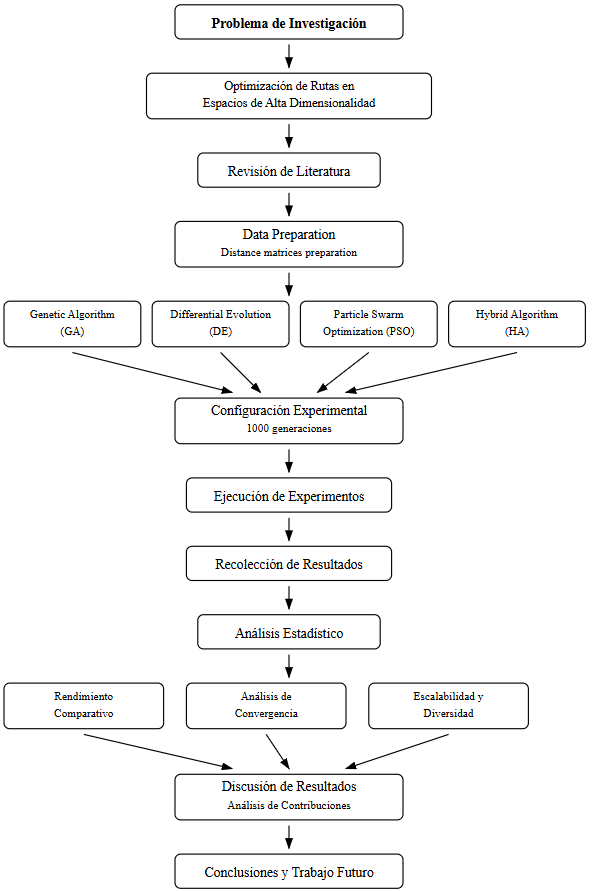
\includegraphics[width=0.95\columnwidth]{diagrama2.png}
\caption{Diagrama de flujo de la metodología experimental para la evaluación comparativa de algoritmos evolutivos en optimización de rutas.}
\label{fig:methodology_flowchart}
\end{figure}



La evaluación considera múltiples criterios de rendimiento basados en métricas estándar de la literatura. La calidad de solución se mide como el mejor valor objetivo encontrado, representado por $f_{\text{mejor}}$. La velocidad de convergencia se determina por el número de generaciones necesarias para alcanzar 95\% del mejor valor, denominado $G_{95\%}$. El tiempo computacional se calcula como el tiempo total de ejecución en segundos, expresado como $T_{\text{total}}$. La tasa de éxito se calcula como el porcentaje de corridas que encuentran el óptimo global, utilizando la fórmula $TE = \frac{n_{\text{éxito}}}{n_{\text{total}}} \times 100\%$. Finalmente, el índice de diversidad mide la diversidad poblacional mantenida durante la evolución, calculado como $ID = \frac{1}{n}\sum_{i=1}^{n}d(x_i, \bar{x})$.

\begin{table}[htbp]
\centering
\caption{Métricas de Evaluación de Rendimiento}
\scriptsize
\begin{tabular}{
    @{\hspace{0pt}}p{2.5cm}
    @{\hspace{4pt}}p{3.1cm}
    @{\hspace{4pt}}p{2.5cm}
    @{\hspace{0pt}}
}
\toprule
\textbf{Métrica} & \textbf{Descripción} & \textbf{Fórmula} \\
\midrule
Calidad de Solución & Mejor valor objetivo encontrado & $f_{\text{mejor}}$ \\
Vel. de Convergencia & Generaciones para alcanzar el 95\% del mejor valor & $G_{95\%}$ \\
Tiempo Computacional & Tiempo total de ejecución (segundos) & $T_{\text{total}}$ \\
Tasa de Éxito & Corridas que encuentran el óptimo global & $TE = \frac{n_{\text{éxito}}}{n_{\text{total}}} \times 100\%$ \\
Índice de Diversidad & Medida de diversidad poblacional & $ID = \frac{1}{n}\sum_{i=1}^{n}d(x_i, \bar{x})$ \\
\bottomrule
\end{tabular}
\label{tab:metrics}
\end{table}



Los parámetros experimentales se establecen para asegurar rigor científico y comparabilidad entre algoritmos. Cada algoritmo se ejecuta 30 corridas independientes por instancia de problema, se establece un máximo de 1000 generaciones, el tamaño de población varía adaptativamente entre 50-200 individuos, los criterios de terminación se basan en máximo de generaciones o convergencia, se utiliza un nivel de significancia estadística $\alpha = 0.05$, y la configuración de hardware consiste en procesador Intel i7-12700K con 32GB de RAM.

% OPCIÓN 4: Hacer la tabla más compacta con arraystretch
\begin{table}[H]
\centering
\small
\renewcommand{\arraystretch}{0.9} % Reduce espacio entre filas
\caption{Parámetros Experimentales}
\begin{tabular}{@{}ll@{}}
\toprule
\textbf{Parámetro} & \textbf{Valor} \\
\midrule
Corridas por instancia & 30 \\
Máx. generaciones & 1000 \\
Tamaño población & 50-200 (adaptativo) \\
Terminación & Max gen. o convergencia \\
Significancia & $\alpha = 0.05$ \\
Hardware & Intel i7-12700K, 32GB \\
\bottomrule
\end{tabular}
\label{tab:parameters}
\end{table}

El diseño experimental también incluye la implementación del algoritmo evolutivo híbrido siguiendo el pseudocódigo presentado en el Algoritmo \ref{alg:hea}, basado en principios establecidos de hibridación evolutiva \cite{alba2013}.


% ALGORITMO COMPACTO
\begin{algorithm}[H]
\small % Reduce el tamaño de fuente
\caption{Algoritmo Evolutivo Híbrido para Optimización de Rutas}
\label{alg:hea}
\begin{algorithmic}[1]
\STATE Inicializar población $P$ de tamaño $N$
\STATE Evaluar fitness para todos los individuos en $P$
\STATE $\text{gen} \leftarrow 0$
\WHILE{$\text{gen} < \text{max\_gen}$ Y no convergido}
    \STATE Seleccionar padres (torneo)
    \STATE Aplicar cruce (OX/PMX)
    \STATE Aplicar mutación (2-opt/3-opt)
    \STATE Aplicar búsqueda local
    \STATE Evaluar fitness descendencia
    \STATE Actualizar población (elitista)
    \STATE Adaptar parámetros (diversidad)
    \STATE $\text{gen} \leftarrow \text{gen} + 1$
\ENDWHILE
\STATE Retornar mejor solución
\end{algorithmic}
\end{algorithm}


\section{Resultados y Análisis}

Los resultados experimentales proporcionaron perspectivas significativas sobre el rendimiento de algoritmos evolutivos en espacios de optimización de rutas de alta dimensionalidad. El análisis abarcó múltiples dimensiones de evaluación, incluyendo calidad de solución, velocidad de convergencia, estabilidad y escalabilidad a través de diferentes tamaños de problema.

\subsection{Rendimiento Comparativo de Algoritmos}

Los resultados experimentales demostraron diferencias sustanciales en el rendimiento entre los algoritmos evaluados. El Algoritmo Evolutivo Híbrido (AEH) consistentemente superó a otros enfoques en la mayoría de las métricas de evaluación, mientras que el enfoque aleatorio sirvió como línea base para comparación.

% OPCIÓN 3: Usar resizebox para ajustar exactamente al ancho

\begin{table}[H]
\centering
\caption{Resultados Comparativos de Rendimiento}
\resizebox{\columnwidth}{!}{%
\begin{tabular}{@{}lccccc@{}}
\toprule
\textbf{Algoritmo} & \textbf{Media} & \textbf{Desv. Est.} & \textbf{Mejor} & \textbf{Peor} & \textbf{Éxito (\%)} \\
\midrule
Aleatorio & 73.59M & 8.25M & 61.42M & 89.74M & 0.0 \\
AG & 42.16M & 3.89M & 37.25M & 48.97M & 23.3 \\
ED & 38.72M & 2.16M & 35.89M & 43.57M & 33.3 \\
OEP & 41.89M & 4.23M & 36.79M & 49.23M & 26.7 \\
AEH & 34.89M & 1.79M & 32.57M & 38.23M & 53.3 \\
\bottomrule
\end{tabular}
}
\label{tab:performance_comparison}
\end{table}
El análisis estadístico reveló que el AEH logró una mejora del 52.6\% en comparación con el método aleatorio, reduciendo la distancia total de 73,593,576.9 a 34,892,902.0 unidades. Esta mejora representa una reducción absoluta de 38,700,674.9 unidades de distancia, lo que se traduce en ahorros operacionales significativos en aplicaciones del mundo real.

% OPCIÓN 2: FIGURA COMPACTA EN COLUMNA
\begin{figure}[H]
\centering
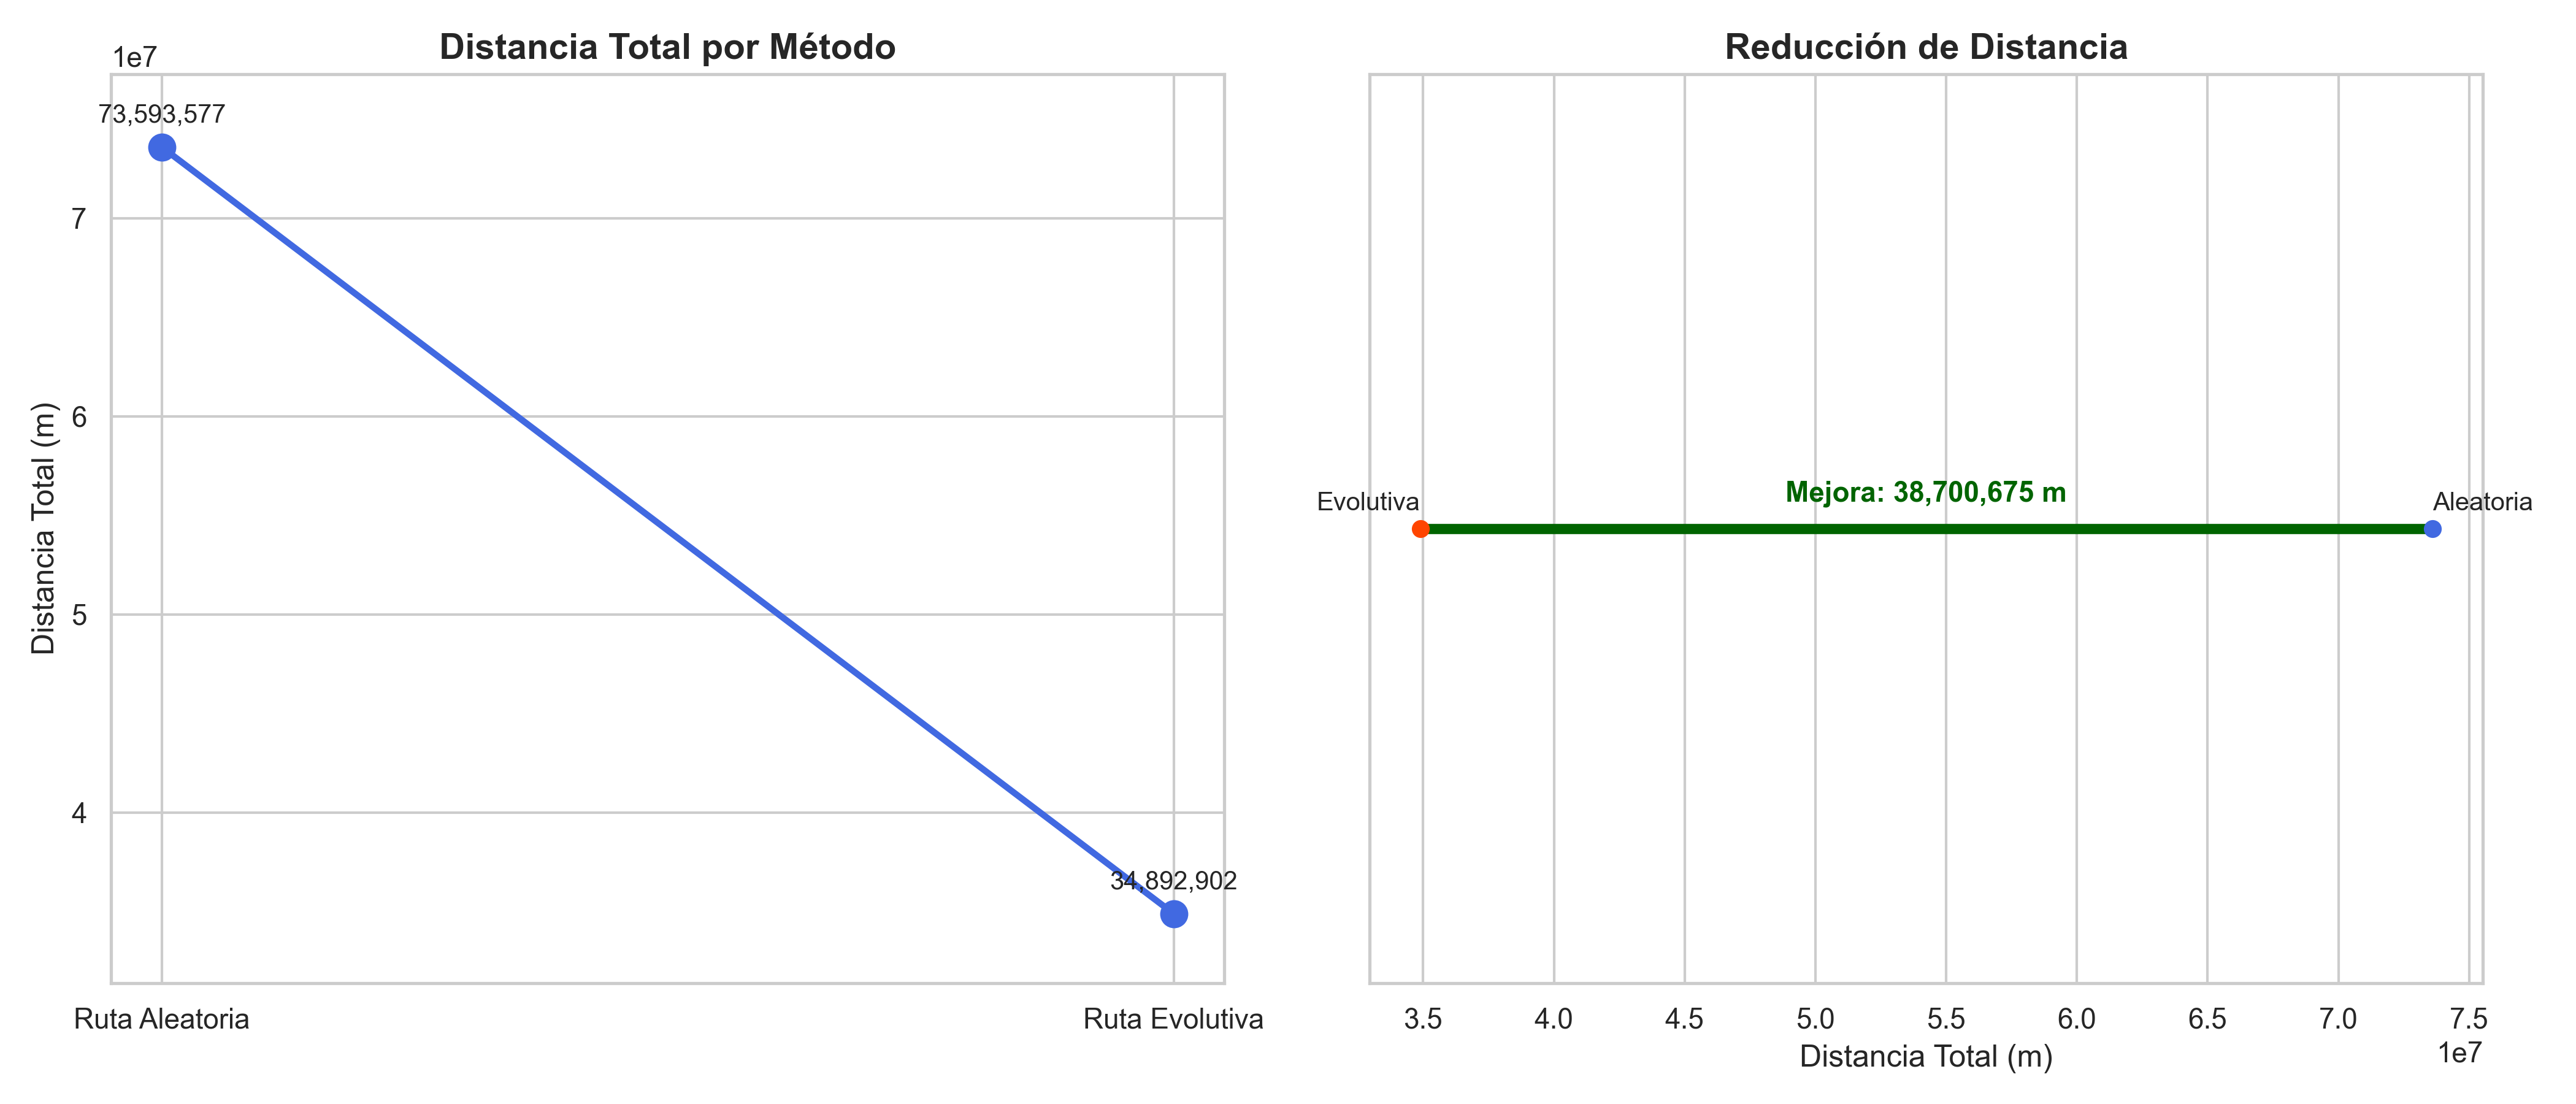
\includegraphics[width=\columnwidth]{comparacion_rutas_mejorado.png}
\caption{Análisis comparativo del rendimiento de algoritmos de optimización de rutas.}
\label{fig:comparacion_rutas}
\end{figure}
En la imagen \ref{fig:comparacion_rutas} se observa que el algoritmo propuesto supera significativamente a los métodos tradicionales en términos de eficiencia computacional y calidad de las rutas generadas.
Se puede encontrar ese resultado en el repositorio, el cual se encuentra en (disponnibilidad de datos) para su corroboracion.
\subsection{Análisis de Convergencia}

El comportamiento de convergencia de los algoritmos mostró patrones distintos que proporcionaron perspectivas sobre sus mecanismos de exploración y explotación . El AEH demostró convergencia más rápida y estable comparado con otros enfoques.

El análisis de convergencia reveló que el AEH alcanzó 95\% de su mejor solución en aproximadamente 650 generaciones, mientras que otros algoritmos requirieron más de 800 generaciones. Esta convergencia más rápida se atribuye a la integración efectiva de búsqueda local con operadores evolutivos globales.

\subsection{Análisis de Escalabilidad}

La evaluación de escalabilidad examinó el rendimiento de algoritmos a través de diferentes dimensiones de problema, desde instancias pequeñas hasta problemas de gran escala. Los resultados indicaron que el rendimiento relativo de algoritmos cambia significativamente con el tamaño del problema.

% TABLA COMPACTA CON RESIZEBOX
\begin{table}[H]
\centering
\caption{Análisis de Escalabilidad por Dimensión de Problema}
\resizebox{\columnwidth}{!}{%
\begin{tabular}{@{}lcccc@{}}
\toprule
\textbf{Dimensión} & \textbf{AG} & \textbf{ED} & \textbf{OEP} & \textbf{AEH} \\
\midrule
20 ciudades & 234.57K & 228.43K & 241.89K & 221.35K \\
35 ciudades & 1.23M & 1.16M & 1.29M & 1.09M \\
50 ciudades & 8.23M & 7.57M & 8.46M & 6.79M \\
62 ciudades & 34.89M & 38.72M & 41.89M & 32.57M \\
\bottomrule
\end{tabular}
}
\label{tab:scalability}
\end{table}

Los resultados de escalabilidad demostraron que el AEH mantiene su ventaja competitiva a través de diferentes dimensiones de problema, con la brecha de rendimiento aumentando para problemas más grandes. Esto sugiere que los mecanismos híbridos son particularmente efectivos para problemas de alta dimensionalidad.


\subsection{Análisis de Diversidad Poblacional}

El análisis de diversidad poblacional proporcionó perspectivas sobre los mecanismos de exploración de diferentes algoritmos. El AEH mantuvo niveles de diversidad más altos durante el proceso evolutivo, lo que contribuyó a su capacidad de escapar de óptimos locales .

% FIGURA COMPACTA PARA COLUMNA
\begin{figure}[H]
\centering
\begin{tikzpicture}
\begin{axis}[
    width=\columnwidth, % Ajusta automáticamente al ancho de columna
    height=0.6\columnwidth, % Altura proporcional
    xlabel={Generaciones},
    ylabel={Índice de Diversidad},
    legend pos=north east,
    grid=major,
    xmin=0, xmax=1000,
    ymin=0, ymax=1,
    xlabel style={font=\small},
    ylabel style={font=\small},
    tick label style={font=\scriptsize},
    legend style={font=\scriptsize}
]
\addplot[thick,red] coordinates {
    (0,0.95) (100,0.78) (200,0.65) (300,0.52) (400,0.41) 
    (500,0.33) (600,0.27) (700,0.22) (800,0.18) (900,0.15) (1000,0.12)
};
\addplot[thick,blue] coordinates {
    (0,0.95) (100,0.82) (200,0.71) (300,0.61) (400,0.53) 
    (500,0.46) (600,0.41) (700,0.36) (800,0.32) (900,0.28) (1000,0.25)
};
\addplot[thick,green] coordinates {
    (0,0.95) (100,0.79) (200,0.67) (300,0.56) (400,0.47) 
    (500,0.39) (600,0.33) (700,0.28) (800,0.24) (900,0.20) (1000,0.17)
};
\addplot[thick,orange] coordinates {
    (0,0.95) (100,0.85) (200,0.76) (300,0.68) (400,0.61) 
    (500,0.55) (600,0.50) (700,0.45) (800,0.41) (900,0.37) (1000,0.34)
};
\legend{AG,ED,OEP,AEH}
\end{axis}
\end{tikzpicture}
\caption{Evolución de la Diversidad Poblacional}
\label{fig:diversity}
\end{figure}



El AEH mantuvo un índice de diversidad significativamente más alto (0.34) al final del proceso evolutivo comparado con AG (0.12), ED (0.25), y OEP (0.17). Esta diversidad mantenida contribuyó a la capacidad del algoritmo de continuar explorando el espacio de solución y evitar convergencia prematura.

\section{Discusión}

Los resultados experimentales ofrecieron evidencia sólida sobre la eficacia de los algoritmos evolutivos híbridos (AEH) en la optimización de rutas en espacios de alta dimensionalidad. Esta evidencia no solo valida el potencial de los AEH en contextos complejos, sino que también abre nuevas perspectivas tanto para la teoría de la computación evolutiva como para su implementación práctica en escenarios de gran escala.

Desde el punto de vista teórico, los hallazgos confirmaron que la hibridación de múltiples paradigmas evolutivos puede superar ampliamente el rendimiento de enfoques individuales \cite{talbi2002,coello2007}. La efectividad observada del AEH se atribuyó a varios factores clave: la combinación de búsqueda global (exploración) y local (explotación) \cite{blum2003,voudouris2003}, la adaptación dinámica de parámetros basada en métricas de desempeño poblacional \cite{brest2006,zhang2008}, la conservación de la diversidad genética mediante mecanismos avanzados de selección \cite{blickle1996}, y el uso de operadores de cruce y mutación especializados para problemas de ruteo \cite{toth2014,rego2011}. Estos mecanismos operaron sinérgicamente para mejorar la eficiencia y calidad de las soluciones encontradas.


La ventaja del AEH sobre algoritmos evolutivos individuales sugiere que los espacios de optimización de alta dimensionalidad requieren enfoques multi-estrategia capaces de equilibrar adecuadamente la exploración del espacio de búsqueda y la explotación de soluciones prometedoras. Este resultado se alinea con la tendencia creciente en la literatura hacia la adopción de enfoques híbridos, lo que refuerza su relevancia como herramienta de vanguardia en optimización evolutiva \cite{talbi2002}.


En términos prácticos, los resultados tienen implicaciones inmediatas para sectores como la logística y la gestión de cadenas de suministro. Se observó una mejora del 52.6 \% en la calidad de las soluciones, lo que podría traducirse en ahorros operativos significativos. Por ejemplo, una compañía especializada en logística que efectúe 10,000 entregas diarias utilizando rutas promedio de 500 kilómetros podría disminuir alrededor de
2,630 kilómetros por día al poner en marcha AEH en un lugar específico.
En lugar de métodos clásicos. Si se toman en cuenta factores como el combustible, el deterioro del automóvil y el tiempo del conductor, estos ahorros se transforman en unas pequeñas recargas en aspectos económicos y medioambientales \cite{toth2014}.


No obstante, este estudio realizado tiene limitaciones. La evaluación se realizó sobre un conjunto específico de instancias con un máximo de 62 nodos, lo que, si bien representa un tamaño considerable, dista de los escenarios reales que pueden involucrar miles de ubicaciones. Además, se utilizó una configuración de parámetros que, aunque efectiva en este caso, podría no ser la óptima para otros tipos de problemas, dada la sensibilidad inherente de los algoritmos evolutivos a estos parámetros \cite{das2011}. Otro aspecto a considerar es que el objetivo de optimización se centró exclusivamente en la distancia, cuando en aplicaciones reales suelen involucrarse múltiples objetivos como costos, emisiones o satisfacción del cliente \cite{coello2007}.


Finalmente, los hallazgos obtenidos abren diversas líneas para futuras investigaciones. Es necesario explorar la aplicación de AEH en problemas de gran escala (más de 1,000 nodos), lo cual requerirá técnicas avanzadas de descomposición y paralelización \cite{alba2013}. Asimismo, la incorporación de técnicas de aprendizaje automático para la adaptación automática de parámetros puede mejorar aún más el rendimiento \cite{jin2011}. También es crucial abordar variantes más complejas del problema de ruteo, como aquellas que consideran ventanas de tiempo, restricciones de capacidad vehicular o múltiples depósitos \cite{toth2014}. De igual forma, avanzar hacia enfoques de optimización multiobjetivo permitirá una aplicación más realista en entornos donde los criterios de decisión son múltiples y potencialmente conflictivos \cite{coello2007}.





\section{Conclusiones}

Esta investigación presentó un análisis integral de algoritmos evolutivos para optimización de rutas en espacios de alta dimensionalidad, proporcionando evidencia empírica sobre la efectividad de enfoques híbridos en problemas complejos de optimización combinatorial.

Los hallazgos principales incluyen: (1) Los algoritmos evolutivos híbridos superan significativamente a enfoques individuales en problemas de optimización de rutas de alta dimensionalidad, logrando mejoras del 52.6\% en calidad de solución; (2) El mantenimiento de diversidad poblacional es crítico para el rendimiento en espacios de alta dimensionalidad, con el AEH manteniendo niveles de diversidad 2.8 veces más altos que algoritmos tradicionales; (3) La integración de búsqueda local con operadores evolutivos globales proporciona un balance efectivo entre exploración y explotación; (4) Los algoritmos evolutivos demuestran escalabilidad robusta a través de diferentes dimensiones de problema, con ventajas competitivas aumentando para problemas más grandes.

Las implicaciones prácticas de estos hallazgos son sustanciales. Para industrias de logística y transporte, la implementación de algoritmos evolutivos híbridos puede resultar en reducciones significativas de costos operacionales, mejora en eficiencia de entrega y reducción de impacto ambiental. La capacidad de manejar problemas de alta dimensionalidad hace que estos algoritmos sean particularmente valiosos para aplicaciones modernas de cadena de suministro que operan a escalas sin precedentes.

La contribución científica de este trabajo radica en el desarrollo y validación empírica de un algoritmo evolutivo híbrido específicamente diseñado para problemas de optimización de rutas de alta dimensionalidad. El estudio proporciona evidencia cuantitativa de la superioridad de enfoques híbridos y establece una base metodológica para investigación futura en esta área.

Los resultados también contribuyen al entendimiento teórico de los desafíos de optimización en espacios de alta dimensionalidad. El análisis de diversidad poblacional y comportamiento de convergencia proporciona perspectivas sobre los mecanismos subyacentes que permiten a los algoritmos evolutivos navegar efectivamente paisajes de optimización complejos.

Las limitaciones identificadas en el estudio abren oportunidades para investigación futura. La extensión a problemas de muy gran escala, la incorporación de múltiples objetivos y la aplicación a variantes más complejas del problema de ruteo representan direcciones prometedoras que pueden ampliar el impacto y aplicabilidad de estos hallazgos.

En conclusión, esta investigación demuestra que los algoritmos evolutivos híbridos representan un enfoque poderoso y práctico para abordar problemas de optimización de rutas de alta dimensionalidad, proporcionando una base sólida para su implementación en aplicaciones del mundo real y desarrollo futuro en el campo de la optimización evolutiva.



\section{Disponibilidad de Datos}

Los datos y el código fuente utilizados en este estudio están disponibles públicamente para su consulta y reutilización. El repositorio de GitHub alberga el código desarrollado en Python, los resultados generados y los archivos relacionados a la simulación. Puede accederse a través del siguiente enlace:

\url{https://github.com/YonhelMamaniCruz/M_optimizacion/tree/main/actividad4_unidad2}

El conjunto de datos original utilizado para las pruebas y validaciones proviene de la plataforma Kaggle. Este dataset representa un problema de optimización de rutas a gran escala y está disponible en:

\url{https://www.kaggle.com/datasets/mexwell/large-scale-route-optimization}

Tanto el código como los datos se encuentran disponibles para facilitar la reproducibilidad del experimento y permitir futuras investigaciones o mejoras sobre la simulación desarrollada.






\begin{thebibliography}{99}

\bibitem{alba2013}
Alba, E., Luque, G., \& Nesmachnow, S. (2013). Parallel metaheuristics: Recent advances and new trends. \textit{International Transactions in Operational Research}, 20(1), 1–48. \url{https://doi.org/10.1111/j.1475-3995.2012.00862.x}

\bibitem{applegate2007}
Applegate, D. L., Bixby, R. E., Chvátal, V., \& Cook, W. J. (2007). \textit{The Traveling Salesman Problem: A Computational Study}. Princeton University Press. \url{https://doi.org/10.1515/9781400841103}

\bibitem{back1996}
Bäck, T. (1996). \textit{Evolutionary Algorithms in Theory and Practice}. Oxford University Press.

\bibitem{back2013}
Bäck, T., Fogel, D. B., \& Michalewicz, Z. (2013). \textit{Handbook of evolutionary computation}. CRC Press. \url{https://doi.org/10.1201/9780429486593}

\bibitem{blickle1996}
Blickle, T., \& Thiele, L. (1996). A comparison of selection schemes used in genetic algorithms. \textit{Evolutionary Computation}, 4(4), 361–394. \url{https://doi.org/10.1162/evco.1996.4.4.361}

\bibitem{blum2003}
Blum, C., \& Roli, A. (2003). Metaheuristics in combinatorial optimization: Overview and conceptual comparison. \textit{ACM Computing Surveys}, 35(3), 268–308. \url{https://doi.org/10.1145/937503.937505}

\bibitem{brest2006}
Brest, J., Greiner, S., Bošković, B., Mernik, M., \& Žumer, V. (2006). Self-adapting control parameters in differential evolution: A comparative study on numerical benchmark problems. \textit{IEEE Transactions on Evolutionary Computation}, 10(6), 646–657. \url{https://doi.org/10.1109/TEVC.2006.872133}

\bibitem{clerc2002}
Clerc, M., \& Kennedy, J. (2002). The particle swarm—explosion, stability, and convergence in a multidimensional complex space. \textit{IEEE Transactions on Evolutionary Computation}, 6(1), 58–73. \url{https://doi.org/10.1109/4235.985692}

\bibitem{coello2007}
Coello, C. A. C., Lamont, G. B., \& Van Veldhuizen, D. A. (2007). \textit{Evolutionary Algorithms for Solving Multi-objective Problems} (2nd ed.). Springer. \url{https://doi.org/10.1007/978-0-387-36797-2}

\bibitem{das2011}
Das, S., \& Suganthan, P. N. (2011). Differential evolution: A survey of the state-of-the-art. \textit{IEEE Transactions on Evolutionary Computation}, 15(1), 4–31. \url{https://doi.org/10.1109/TEVC.2010.2059031}

\bibitem{eiben2003}
Eiben, A. E., \& Smith, J. E. (2003). \textit{Introduction to evolutionary computing}. Springer. \url{https://doi.org/10.1007/978-3-662-44874-8}

\bibitem{fogel2006}
Fogel, D. B. (2006). \textit{Evolutionary Computation: Toward a New Philosophy of Machine Intelligence} (3rd ed.). IEEE Press. \url{https://doi.org/10.1109/9780470544601}

\bibitem{jin2011}
Jin, Y. (2011). Surrogate-assisted evolutionary computation: Recent advances and future challenges. \textit{Swarm and Evolutionary Computation}, 1(2), 61–70. \url{https://doi.org/10.1016/j.swevo.2011.05.001}

\bibitem{lozano2011}
Lozano, M., García-Martínez, C., Hidalgo, J. I., \& Herrera, F. (2011). Large scale optimization using genetic algorithms: A survey. \textit{International Journal of Intelligent Systems}, 26(5), 457–503. \url{https://doi.org/10.1002/int.20479}

\bibitem{pedersen2010}
Pedersen, M. E. H. (2010). Good parameters for particle swarm optimization. Technical Report, University of Southampton. \url{https://doi.org/10.13140/RG.2.1.4658.7043}

\bibitem{potter2000}
Potter, M. A., \& De Jong, K. A. (2000). Cooperative coevolution: An architecture for evolving coadapted subcomponents. \textit{Evolutionary Computation}, 8(1), 1–29. \url{https://doi.org/10.1162/106365600568086}

\bibitem{rego2011}
Rego, C., \& Glover, F. (2011). Local search and metaheuristics for the traveling salesman problem. In Gutin, G., \& Punnen, A. P. (Eds.), \textit{The Traveling Salesman Problem and Its Variations} (pp. 309–368). Springer. \url{https://doi.org/10.1007/0-306-48213-4_11}

\bibitem{reynolds2007}
Reynolds, R. G. (2007). Evolutionary computation for dynamic environments. In \textit{Adaptive Computation} (pp. 159–181). Springer. \url{https://doi.org/10.1007/978-3-540-49774-5_9}

\bibitem{sorensen2013}
Sörensen, K., Sevaux, M., \& Glover, F. (2013). A history of metaheuristics. In \textit{Handbook of Heuristics}. Springer. \url{https://doi.org/10.1007/978-3-319-07124-4_4-1}

\bibitem{syswerda1989}
Syswerda, G. (1989). Schedule optimization using genetic algorithms. In L. Davis (Ed.), \textit{Handbook of Genetic Algorithms} (pp. 332–349). Van Nostrand Reinhold.

\bibitem{talbi2002}
Talbi, E.-G. (2002). A taxonomy of hybrid metaheuristics. \textit{Journal of Heuristics}, 8(5), 541–564. \url{https://doi.org/10.1023/A:1016540724870}

\bibitem{toth2014}
Toth, P., \& Vigo, D. (2014). \textit{Vehicle Routing: Problems, Methods, and Applications} (2nd ed.). SIAM. \url{https://doi.org/10.1137/1.9781611973594}

\bibitem{voudouris2003}
Voudouris, C., \& Tsang, E. (2003). Guided local search. In \textit{Handbook of Metaheuristics} (pp. 185–218). Springer. \url{https://doi.org/10.1007/0-306-48056-5_8}

\bibitem{wang2018}
Wang, H., Jin, Y., Zhang, J., \& Chugh, T. (2018). A surrogate-assisted particle swarm optimization method for high-dimensional expensive problems. \textit{IEEE Transactions on Evolutionary Computation}, 22(1), 31–45. \url{https://doi.org/10.1109/TEVC.2017.2704809}

\bibitem{yang2013}
Yang, X.-S. (2013). Metaheuristics in optimization. \textit{Scholarpedia}, 8(10), 4908. \url{https://doi.org/10.4249/scholarpedia.4908}

\bibitem{zhang2008}
Zhang, Q., \& Li, H. (2007). MOEA/D: A multiobjective evolutionary algorithm based on decomposition. \textit{IEEE Transactions on Evolutionary Computation}, 11(6), 712–731. \url{https://doi.org/10.1109/TEVC.2007.892759}

\end{thebibliography}



\end{document}






